\documentclass[14pt]{article} % use larger type; default would be 10pt

\usepackage{ctex}
%%% Examples of Article customizations
% These packages are optional, depending whether you want the features they provide.
% See the LaTeX Companion or other references for full information.

\usepackage{listings}
\newfontfamily\courier{Courier New}
\lstset{linewidth=1.1\textwidth,
	numbers=left,
	basicstyle=\small\courier,
	numberstyle=\tiny\courier,
	keywordstyle=\color{blue}\courier,
	commentstyle=\it\color[cmyk]{1,0,1,0}\courier, 
	stringstyle=\it\color[RGB]{128,0,0}\courier,
	frame=single,
	breaklines,
	extendedchars=false, 
	xleftmargin=2em,xrightmargin=2em, aboveskip=1em,
	tabsize=4, 
	showspaces=false
	basicstyle=\small\courier
}

%%% PAGE DIMENSIONS
\usepackage{geometry} % to change the page dimensions
\geometry{a4paper} % or letterpaper (US) or a5paper or....
% \geometry{margin=2in} % for example, change the margins to 2 inches all round
% \geometry{landscape} % set up the page for landscape
%   read geometry.pdf for detailed page layout information

\usepackage{graphicx} % support the \includegraphics command and options
\usepackage{pdfpages}

% \usepackage[parfill]{parskip} % Activate to begin paragraphs with an empty line rather than an indent

%%% PACKAGES
\usepackage{booktabs} % for much better looking tables
\usepackage{array} % for better arrays (eg matrices) in maths
\usepackage{paralist} % very flexible & customisable lists (eg. enumerate/itemize, etc.)
\usepackage{verbatim} % adds environment for commenting out blocks of text & for better verbatim
\usepackage{subfig} % make it possible to include more than one captioned figure/table in a single float
% These packages are all incorporated in the memoir class to one degree or another...

%%% HEADERS & FOOTERS
\usepackage{fancyhdr} % This should be set AFTER setting up the page geometry
\pagestyle{fancy} % options: empty , plain , fancy
\renewcommand{\headrulewidth}{0pt} % customise the layout...
\lhead{}\chead{}\rhead{}
\lfoot{}\cfoot{\thepage}\rfoot{}

%%% SECTION TITLE APPEARANCE
\usepackage{sectsty}
\allsectionsfont{\sffamily\mdseries\upshape} % (See the fntguide.pdf for font help)
% (This matches ConTeXt defaults)

%%% ToC (table of contents) APPEARANCE
\usepackage[nottoc,notlof,notlot]{tocbibind} % Put the bibliography in the ToC
\usepackage[titles,subfigure]{tocloft} % Alter the style of the Table of Contents
\usepackage{amsfonts}
\usepackage{amsmath}
\renewcommand{\cftsecfont}{\rmfamily\mdseries\upshape}
\renewcommand{\cftsecpagefont}{\rmfamily\mdseries\upshape} % No bold!
\usepackage{bytefield}
%%% END Article customizations

%%% The "real" document content comes below...
\title{\LARGE \bf 计算机网络实验一\\
实\ 验\ 报\ 告}

\author{2017211305班级\ 于海鑫}
\date{} % Set empty date
\begin{document}
%\maketitle

\includepdf[pages={1}]{NETWORK.pdf}
\section{实验目的}
利用所学数据链路层原理,自己设计一个滑动窗口协议,在仿真环境下编程实现有噪音信道环境下
两站点之间无差错双工通信。信道模型为 8000bps 全双工卫星信道,信道传播时延 270 毫秒,信道误码率
为 10-5,信道提供字节流传输服务,网络层分组长度固定为 256 字节。

通过该实验,进一步巩固和深刻理解数据链路层误码检测的 CRC 校验技术,以及滑动窗口的工作机
理。滑动窗口机制的两个主要目标:(1) 实现有噪音信道环境下的无差错传输; (2)充分利用传输信道的带
宽。在程序能够稳定运行并成功实现第一个目标之后,运行程序并检查在信道没有误码和存在误码两种
情况下的信道利用率。为实现第二个目标,提高滑动窗口协议信道利用率,需要根据信道实际情况合理
地为协议配置工作参数,包括滑动窗口的大小和重传定时器时限以及 ACK 搭载定时器的时限。这些参数
的设计,需要充分理解滑动窗口协议的工作原理并利用所学的理论知识,经过认真的推算,计算出最优
取值,并通过程序的运行进行验证。

在本实验中,可选的协议类型为“不
搭载 ACK 的 Go-Back-N 协议”,“使用搭载 ACK 技术的 Go-Back-N 协议”,“选择重传协议”。本次实验中选取了后两种协议进行实现,并对“选择重传协议”进行了少许改进以适应不同环境的信道。

两个协议的算法流程图一致且与书中流程无区别,在此给出网络上的流程图:

\begin{figure}[!htbp]        
	\center{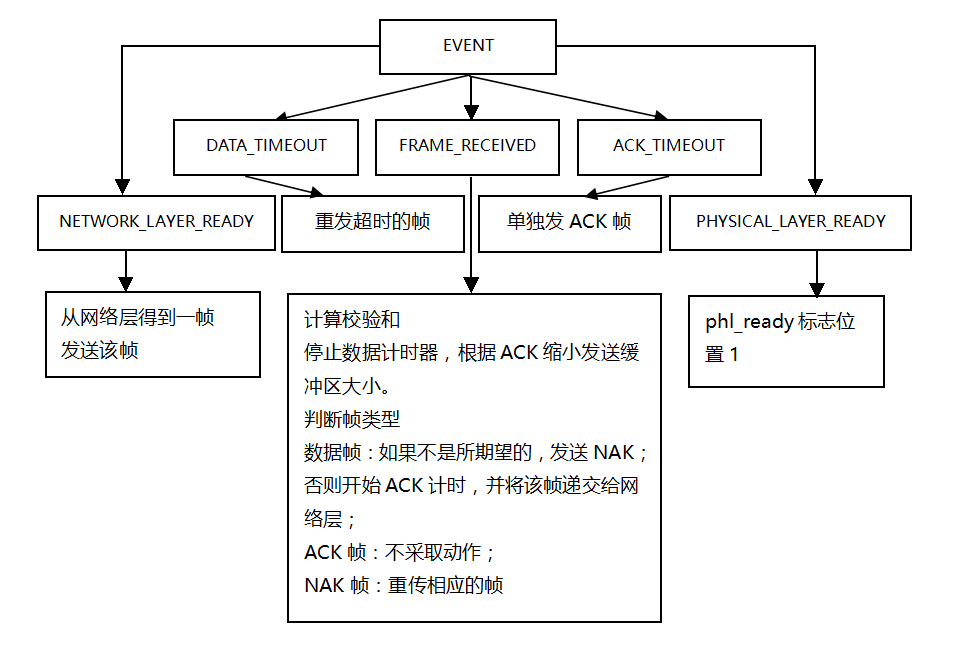
\includegraphics[width=15cm]  {NETWORK.png}}        
	\caption{\label{1} 协议算法流程图 \textbf{Source:} Internet}      
\end{figure}

\section{软件环境}
本实验提供的资料包可以在 Windows 以及 32 位 Linux 上运行,本实验报告中选择的环境为 64 位 Windows 10 以及 Microsoft Visual Studio Community 2019 集成开发环境。

\section{搭载 ACK 的 Go-Back-N 协议}
\subsection{实现}
在该协议中使用的数据帧格式如下:
\begin{center}
\begin{bytefield}{32}
	\bitbox{8}{KIND} & \bitbox{8}{ACK} & \bitbox{8}{SEQ} & \bitbox{8}{DATA}\\
	\wordbox[lrt]{1}{DATA} \\
	\skippedwords \\
	\wordbox[lrb]{1}{} \\
	\wordbox{1}{PADDING}
\end{bytefield}
\end{center}
ACK/NAK 帧的格式如下:
\begin{center}
	\begin{bytefield}{34}
		\bitbox{8}{KIND} & \bitbox{8}{ACK} & \bitbox{8}{SEQ}
	\end{bytefield}
\end{center}
各个字段的含义如下:
\begin{itemize}
	\item KIND: 包的类型,取值为 $FRAME\_DATA$、 $FRAME\_ACK$ 以及 $FRAME\_NAK$
	\item ACK:ACK
	\item SEQ:包的序号
	\item DATA:数据,最多 256 字节
	\item PADDING: CRC 校验和
\end{itemize}

程序的大部分实现与书中别无二致,在此不再赘述。需要注意的是程序中存在三个参数 $DATA\_TIME$(数据的超时时间),$ACK\_TIMER$(ACK 的超时时间) 和 $MAX\_SEQ$(窗口大小) 的取值需要通过实验以获得最佳结果。经过实验我们发现信道的延迟并非为标称的 270ms,实际延时大约在 276ms 左右,大约是因为程序从物理层获取数据也要花费一部分时间。因此我们选取如下参数作为最终结果:
$$DATA\_TIME = 2000ms$$
$$ACK\_TIMER = 300ms$$
$$MAX\_SEQ = 31$$

\subsection{运行结果}
根据性能测试表中的要求运行程序后的结果如下。

\begin{table}[!htbp]
	\caption{Go-back-N 算法测试结果}\label{gbn} \centering
	\begin{tabular}{cccc}
		\toprule[1.5pt]
		\makebox[0.3\textwidth][c]{参数}	&  \makebox[0.1\textwidth][c]{运行时间} &
		\makebox[0.2\textwidth][c]{线路利用率(A)} & \makebox[0.2\textwidth][c]{线路利用率(B)} \\ \midrule[1pt]
		\textendash utopia & 1745.818 & 52.98\% & 96.97\% \\
		无 & 2668.260 & 36.06\% & 72.29\% \\
		\textendash flood \textendash utopia & 1447.494 & 96.97\% & 96.97\% \\
		\textendash flood & 1312.355 & 63.93\% & 65.33\% \\
		\textendash flood  \textendash ber=1e-4 & 1438.589 & 22.14\% & 21.90\% \\
		\bottomrule[1.5pt]
	\end{tabular}
\end{table}

可以发现,回退 N 协议的效率不是很理想。我们也不将该协议作为实现的重点,而是将之作为与选择重传协议对比的标准。

\section{选择重传协议}
\subsection{实现}
在该协议中使用的数据包格式与上一版本一致。主要改动在于实现的算法。此处实现的算法为教科书上提到的选择重传协议算法的改进版,其主要改进为减小了 NAK/ACK 包的大小。核心改进代码如下:
\begin{lstlisting}[language=C]
static void put_frame_crc(unsigned char* frame, int len) {
	*(unsigned int*)(frame + len) = crc32(frame, len);
	send_frame(frame, len + 4);
	phl_ready = false;
}

static void put_frame_naive(unsigned char* frame) {
	send_frame(frame, 3);
}

static void send_link_frame(frame_type fk, seq_nr frame_nr, seq_nr frame_expceted, struct buffer buffer[]) {
	struct FRAME s;
	s.kind = fk;
	if (fk == FRAME_DATA) {
		memcpy(s.data, buffer[frame_nr % NR_BUFS].buf, buffer[frame_nr % NR_BUFS].length);
		s.seq = frame_nr;
		dbg_frame("Send DATA %d %d, ID %d\n", frame_nr,
		((frame_expceted + MAX_SEQ) % (MAX_SEQ + 1)), *(short*)s.data);
	}
	s.ack = ((frame_expceted + MAX_SEQ) % (MAX_SEQ + 1));
	if (fk == FRAME_NAK) {
		dbg_frame("Send NAK %d\n", frame_expceted);
		no_nak = false;
	}
	if (fk == FRAME_ACK || fk == FRAME_NAK) {
	put_frame_naive((unsigned char*)&s);
	} else
		put_frame_crc((unsigned char*)&s, 3 + buffer[frame_nr % NR_BUFS].length);
	if (fk == FRAME_DATA) {
		start_timer(frame_nr % NR_BUFS, DATA_TIMER);
	}
	stop_ack_timer();
}
\end{lstlisting}

除此之外,为了确保在高错误率的信道环境中不因为多次重传而降低信道的传输效率,我实现了根据网络状况自适应调整计时器等待时长。其核心代码如下:
\begin{lstlisting}[language=C]
if ((error_received << 22) < bits_received) {
	low_error = true;
} else {
	low_error = false;
}

if (bits_received > 0x3f3f3f3f) {
	bits_received >>= 20;
	error_received >>= 20;
}

if (low_error) {
	DATA_TIMER = 3500;
} else {
	DATA_TIMER = 5000;
}
\end{lstlisting}
因为协议的修改,协议的参数自然也进行了相应的修改。在选择重传协议中使用的参数如下:
$$DATA\_TIME = AUTO$$
$$ACK\_TIMER = 666ms$$
$$MAX\_SEQ = 31$$
$$NR\_BUFS = \frac {MAX\_SEQ + 1} {2}$$
\subsection{运行结果}
根据性能测试表中的要求运行程序后的结果如下。

\begin{table}[!htbp]
	\caption{选择重传算法测试结果}\label{sr} \centering
	\begin{tabular}{cccc}
		\toprule[1.5pt]
		\makebox[0.3\textwidth][c]{参数}	&  \makebox[0.1\textwidth][c]{运行时间} &
		\makebox[0.2\textwidth][c]{线路利用率(A)} & \makebox[0.2\textwidth][c]{线路利用率(B)} \\ \midrule[1pt]
		\textendash utopia & 1135.255 & 54.25\% & 96.97\% \\
		无 & 1361.205 & 52.16\% & 94.17\% \\
		\textendash flood \textendash utopia & 1707.305 & 96.97\% & 96.97\% \\
		\textendash flood & 1569.032 & 94.59\% & 94.29\% \\
		\textendash flood  \textendash ber=1e-4 & 1244.861 & 57.11\% & 55.56\% \\
		\bottomrule[1.5pt]
	\end{tabular}
\end{table}

可以注意到,与回退 N 协议相比,选择重传算法的效率有了巨大的提升。测试结果与参考测试结果的差距也不过 1\%,足以表明选择重传算法之高效。

\section{结果分析}
\subsection{正确性与鲁棒性}
显然,实现的两个程序都可以正确的传输数据,并可以长时间运行。
\subsection{参数的选择}
窗口的计算过程如下:
\begin{equation}
\left\{
\begin{array}{lr}
t_p = 270ms, &  \\
t_f = \frac {260 \times 8 + 8 + 2\times \log_2 (2W)}{8000}, &\\
\frac{W t_f}{2t_f + 2_tp} \geq 1&  
\end{array}
\right.
\end{equation}

求解得知 $W > 4$ 即可,但是根据实验可以发现实际上 4  的窗口大小很好的制约了窗口的拓展。因此我们将窗口大小设为了 32。

计时器的值通过多次实验给出,结果在上文中已经描述过了。
\subsection{理论最优信道利用率}
假设当前信道的误码率为$p$,则对于一个 263 Byte 的包,其一次成功发送的概率为:
$$P = (1 - p)^{263 \times 8} = (1 - p)^{2102}$$
假设一帧需要重传的次数为随机变量$X$,对之取期望,有
$$E[X] = \sum_{i = 1}^{\infty} i \times (1 - P)^{i - 1}P = \frac{1}{P}$$
因此理论最优信道利用率为:
$$\eta  = \frac{256}{263\times E[X]}$$
带入数据,得知当 $p = 10^{-5}$ 时,有
$$\eta = 95.31\%$$
而当 $p = 10^{-4}$ 时,有
$$\eta = 78.84\%$$
\subsection{实验结果分析}
实验结果的表格为表~\ref{gbn}~以及表~\ref{sr}~。回退N协议的实现因为只是作为一个比较,实现的比较随意,故利用率和参考的利用率相比低了不少。选择重传协议前四种情况与参考利用率差距不大,但是当误码率为 $10^-4$ 时效率仅为 55\%,远远不如参考结果。
究其原因,为\textbf{无意义的重传太多},日志文件中随处可见如下这种连续的超时重传:
\begin{lstlisting}
1238.695 ---- DATA 5 timeout
1238.695 Send DATA 5 2, ID 22757
1238.744 Recv DATA 2 3, ID 12690
1238.952 ---- DATA 6 timeout
1238.953 Send DATA 6 2, ID 22758
1239.002 Recv DATA 0 3, ID 12688
1239.228 ---- DATA 7 timeout
1239.228 Send DATA 7 2, ID 22759
1239.276 ****RECEIVER ERROR, BAD CRC CHECKSUM****
1239.531 Recv DATA 4 3, ID 12692
1239.610 ---- DATA 4 timeout
1239.611 Send DATA 4 2, ID 22756
1239.754 ---- DATA 8 timeout
1239.755 Send DATA 8 2, ID 22760
1239.804 ****RECEIVER ERROR, BAD CRC CHECKSUM****
1240.011 ---- DATA 9 timeout
1240.012 Send DATA 9 2, ID 22761
1240.061 Recv DATA 3 3, ID 12691
1240.062 .... 2692 packets received, 4450 bps, 55.63%, Err 920 (1.0e-04)
1240.284 ---- DATA 10 timeout
1240.287 Send DATA 10 4, ID 22762
1240.336 Recv DATA 6 3, ID 12694
1240.337 Send NAK 5
1240.530 ---- DATA 11 timeout
1240.530 Send DATA 11 4, ID 22763
1240.578 ****RECEIVER ERROR, BAD CRC CHECKSUM****
1240.801 ---- DATA 12 timeout
1240.801 Send DATA 12 4, ID 22764
1240.849 Recv DATA 8 3, ID 12696
1241.073 ---- DATA 13 timeout
1241.074 Send DATA 13 4, ID 22765
1241.107 Recv DATA 9 3, ID 12697
1241.331 ---- DATA 14 timeout
1241.332 Send DATA 14 4, ID 22766
1241.380 Recv DATA 10 9, ID 12698
1241.384 Recv NAK 9
1241.384 Send DATA 10 4, ID 22762
1241.593 ---- DATA 15 timeout
1241.594 Send DATA 15 4, ID 22767
1241.658 Recv DATA 5 10, ID 12693
\end{lstlisting}

这类问题的解决方法有两种:其一是增加 NAK 帧的发送次数,催促发送方尽快重发出错的帧;其二是彻底弃用累积确认,对每个帧单独发送 ACK。因为时间问题,并未实现这两个解决方法。

\section{研究与探索的问题}
\subsection{CRC 的校验能力}
本次实验采用的 CRC 校验方案为 CRC-32,与 IEEE 802.3 以太网校验和生成多项式相同。生成多项
式为:
$$x^{32}+x^{26}+x^{23}+x^{22}+x^{16}+x^{12}+x^{11}+x^{10}+x^{8}+x^{7}+x^{5}+x^{4}+x^{2}+x^{1}+1$$
CRC 校验和的生成有硬件产生和软件计算两种方式。硬件产生通过移位寄存器电路实现。教科书中
给出了计算 CRC 校验和的方法:根据 CRC 多项式得到一个 33 比特的除数;将待校验的 n 字节帧理解为
8n 比特的二进制数,在后面追加 32 个 0 构成被除数;然后进行“模 2”除法,得到 32 比特余数作为校
验和。由于一般通用的 CPU 未提供按位“模 2”除法的指令,需要通过软件模仿这种除法。目前,通过
软件计算的方式求校验和,一般用查表并叠加的方式,将逐比特进行的模 2 除法改造为更高效率的逐字
节进行模 2 除法。从传输错误的概率为2的-32次方,几乎接近于0,因此没有必要增加成本再去达到理论上为0的错误率。另外,如果CRC校验错误而导致给网络层传输了错误数据,那么网络层也应该可以通过它的校验方式发现错误,采取重传,因此能够进一步保证传输的正确性。
\subsection{软件测试的问题}
除去默认的信道,实验还提供了四个参数,各个参数的效果如下:
\begin{itemize}
	\item \textbf{\textendash utopia}\ 打开该选项将获得一个无误码的信道(所谓乌托邦式)。该选项可以用于测试协议的最大吞吐能力,其效率只与帧的格式相关。
	\item \textbf{\textendash flood}\ 洪水模式。本站网络层有无穷量分组流及时供应给数据链路
	层发送可以用于测试协议的抗压能力以及最大输出能力。
	\item \textbf{\textendash ber=$1e^-4$}\ 高误码率的信道,着重考察协议的重传机制的效果。
	\item \textbf{default}\ 站点 A 以较平缓方式断断续续不停产生分
	组流,站点 A 以 100 秒为周期发一段停一段。综合考察协议的性能以及参数的选取效果。
\end{itemize}
\section{总结和心得体会}
本次实验实际的上机时间为 6 小时,主要时间在于运行程序等待结果并进行调参的时间。编程工具上因为使用了最新的 Visual Stdio 2019,需要对解决方案进行升级。其余主要时间就是将书上的伪代码翻译为使用老师提供的库的 C 代码。总体来说,难度不是过大。

\appendix
\section{附录:数据结构}
各个参数的命名与书上几乎一致。
\begin{lstlisting}[language=C]
/* FRAME kind */
#define FRAME_DATA 1
#define FRAME_ACK  2
#define FRAME_NAK  3

#define MAX_SEQ 0x1f
#define NR_BUFS ((MAX_SEQ + 1) / 2)
#define MAX_PKT 256
#define ACK_TIMER 666

#define inc(k) (k = (k + 1) & MAX_SEQ)

typedef unsigned char seq_nr; // frame nubmber
typedef unsigned char frame_type; // frame type

struct FRAME {
	unsigned char kind; /* FRAME_DATA */
	unsigned char ack;
	unsigned char seq;
	unsigned char data[MAX_PKT];
	unsigned int padding;
};

struct buffer {
	unsigned char buf[MAX_PKT];
	size_t length;
};

seq_nr ack_expected = 0;
seq_nr next_frame_to_send = 0;
seq_nr frame_expected = 0;
seq_nr nbuffered = 0;
seq_nr r_seq = 0, r_ack = 0;
seq_nr too_far = NR_BUFS;
int event, arg, len;
struct FRAME r;
struct buffer out_buf[NR_BUFS] = {0};
struct buffer in_buf[NR_BUFS] = {0};
bool arrived[NR_BUFS];
for (int i = 0; i < NR_BUFS; i++)
	arrived[i] = false;
\end{lstlisting}
\end{document}